\documentclass[a4paper,12pt,twoside,openright,titlepage]{book}
\usepackage[utf8]{inputenc}
\usepackage[T1]{fontenc}
\usepackage[english]{babel}
\usepackage{amsmath,amsthm,amssymb}
\usepackage[colorlinks=true]{hyperref}
\usepackage{graphicx}
\usepackage{pdfpages}
\usepackage{amsmath}
\usepackage{lastpage}
\usepackage{spverbatim}
\usepackage{listings}
\usepackage{longtable}
\usepackage{subfig}
\usepackage{hyperref}
\usepackage{float}
\usepackage{siunitx}
\usepackage{multicol}

\usepackage[toc,page]{appendix}


\usepackage{color}
 
\definecolor{codegreen}{rgb}{0,0.6,0}
\definecolor{codegray}{rgb}{0.5,0.5,0.5}
\definecolor{codepurple}{rgb}{0.58,0,0.82}
\definecolor{backcolour}{rgb}{0.95,0.95,0.92}
 
\lstdefinestyle{mystyle}{
    backgroundcolor=\color{backcolour},   
    commentstyle=\color{codegreen},
    keywordstyle=\color{magenta},
    numberstyle=\tiny\color{codegray},
    stringstyle=\color{codepurple},
    basicstyle=\footnotesize,
    breakatwhitespace=false,         
    breaklines=true,                 
    captionpos=b,                    
    keepspaces=true,                 
    numbers=left,                    
    numbersep=5pt,                  
    showspaces=false,                
    showstringspaces=false,
    showtabs=false,                  
    tabsize=2
}
 
\lstset{style=mystyle}



\graphicspath{fig/}

\begin{document}
\frontmatter

\begin{titlepage} % Suppresses displaying the page number on the title page and the subsequent page counts as page 1
	\newcommand{\HRule}{\rule{\linewidth}{0.5mm}} % Defines a new command for horizontal lines, change thickness here
	
	\center % Centre everything on the page
	
	%------------------------------------------------
	%	Headings
	%------------------------------------------------
	
	\textsc{\LARGE Fróðskaparsetur Føroya}\\[1.5cm] % Main heading such as the name of your university/college
	
	\textsc{\Large 5025.16 KT-verkætlan (2018)}\\[0.5cm] % Major heading such as course name
	
	\textsc{\large Arduino Project}\\[0.5cm] % Minor heading such as course title
	
	%------------------------------------------------
	%	Title
	%------------------------------------------------
	
	\HRule\\[0.4cm]
	
	{\huge\bfseries Radar}\\[0.4cm] % Title of your document
	
	\HRule\\[1.5cm]
	
	%------------------------------------------------
	%	Author(s)
	%------------------------------------------------
	
	\begin{minipage}{0.4\textwidth}
		\begin{flushleft}
			\large
			\textit{Author}\\
			Helgi \textsc{Poulsen} % Your name
		\end{flushleft}
	\end{minipage}
	~
	\begin{minipage}{0.4\textwidth}
		\begin{flushright}
			\large
			\textit{Author}\\
			Anna \textsc{Thomsen} % Author's name
		\end{flushright}
	\end{minipage}
	~
	\begin{minipage}{0.4\textwidth}
		\begin{center}	
			\large
			\textit{Supervisor}\\
			Benadikt \textsc{Joensen} % Author's name
		\end{center}
	\end{minipage}
	
	% If you don't want a supervisor, uncomment the two lines below and comment the code above
	%{\large\textit{Author}}\\
	%John \textsc{Smith} % Your name
	
	%------------------------------------------------
	%	Date
	%------------------------------------------------
	
	\vfill\vfill\vfill % Position the date 3/4 down the remaining page
	
	{\large\today} % Date, change the \today to a set date if you want to be precise
	
	%------------------------------------------------
	%	Logo
	%------------------------------------------------
	
	%\vfill\vfill
	%\includegraphics[width=0.2\textwidth]{placeholder.jpg}\\[1cm] % Include a department/university logo - this will require the graphicx package
	 
	%----------------------------------------------------------------------------------------
	
	\vfill % Push the date up 1/4 of the remaining page
	
\end{titlepage}
{
  \hypersetup{linkcolor=black}
  \tableofcontents
}
\newenvironment{abstract}%
{\cleardoublepage\addcontentsline{toc}{chapter}{Abstract}\null\vfill\begin{center}%
\bfseries\abstractname\end{center}}%
{\vfill\null}
\begin{abstract}
Kunningartøkni, programmering og tól/dimsar er blivi lættari og lættari atkomuligt fyri forbrúkaran, also øll eiga onkran lítlan dims. Við alnótuni og microteldum, sum Arduino, kunnu øll gera teirra egnu dimsar.  

Hetta projektið snýr seg um at nýta ein Arduino Uno og fleiri smærri komponentar, til at gera ein lítlan einklan radara. Hetta fyri at skilja tey grundleggjandi tingini ísmb. við programmering og at nýta tað til at gera okkurt funktionelt ting, td. ein dims. 
\end{abstract}

\cleardoublepage\addcontentsline{toc}{chapter}{Contents}


\chapter{Foreword}
In the course 5025.16 KT-verkætlan (2018) we are required to make a project of our choosing, to learn how to create a project and write a report about it. This is done to prepare us to the bachelor project.

In this project we have included everything from building the radar, writing and understanding the code and showing how tests can be made from a ultrasonic sensor.

Doing this project helped us to understand and enhance our knowledge in starting a project, finding information about it and in the end write a report about it in LaTeX. Through this report we come to know about importance of team work and role of devotion towards the work.

\addcontentsline{toc}{section}{Acknowledgement}
\section*{Acknowledgement} 
In any project it is very important to have guidance. In this project we had Mr.Benadikt Joensen as our supervisor. We are very grateful for the help he provided us through this project from start to finish. 

We also want to give all our classmates that helped us with various problems that we encountered. 

We also want to give a special thanks to our classmates Fróði H. Joensen and Bergur I. Johansen for providing smart solutions when it came to the coding. 
\mainmatter
\chapter{Introduction}
In this project we are going to work with an Arduino Uno microcomputer and a variety of components to create a small-scale radar. This to get a small understanding of the Arduino and the possibilities it comes with.  

The Arduino programming comes with some number of pre-set libraries, but they haven't always got the most satisfying codes for the project. Therefore, one has sometimes to write new codes, which we will also see in this project. 

From this point on $on$ and $off$ are going to be used instead of $start$ and $stop$. This to indicate that the radar is being turned on and off, but the Arduino Uno itself is not being turned on and off. 
\chapter{Problem description and statement}
The object of this project is to get a small, but basic understanding of Arduino hardware and software, this to be able to create a small working piece of machinery. After some thinking and discussing this machinery is going to be a small radar, which the measurements will be shown on a small screen and also using LED's to indicate an object nearby. Throughout this project there is a learning curve incorporated, where the beginning is a rock bottom, we need to learn Arduino programming and how to utilize it. Thereafter it is possible to start to build the actual project or said in other words, we start with turning on a small LED and expand it into a small-scale radar. Even making some thoughts about how it can be upgraded in the future and possible improvements. 

The radar is built in such a way, that it sends and receives signal in all directions, $360$ degrees, anything else would be useless. However, when creating a small school project, it's a highly simplified version and it has its limitations. The radar has a view range of about $180$ degrees and can only check one degree at the time and is only accurate on static objects.
\chapter{Radar}
A radar, well what does it do and why we use it? 

The challenge of seeing objects and estimating a distance to these objects, has been vastly minimized by the invention of the radar. Not only does the radar tell you that there is an object, but it also tells you in which direction and at what distance the object is. This has shown to be very use full onboard ships and aeroplanes, but also on land, at stations monitoring ship and air traffic, airports etc. While placed on land, the main purpose of the radar is to detect ship traffic and air traffic. But when a radar is placed on for example a ship, its main purpose is to detect other ships and/or objects within the sailing path, so that the ship doesn't collide, it prevents accidents. 

The radar is the eyes and ears of the navigator. It has a 360-degree view and can detect moving objects as well as still standing objects. It gives you the direction, distance and speed of the object, no matter how big or small the object is, but of course depending on the type of radar and the use.  

A radar is based on a radio transmitter and a receiver, therefore the name radar (Radio Detection And Ranging). It uses a very high frequency, much higher than any television or radio signal, this to prevent distortion from other radio signals. When in function it sends out small electromagnetic pulses, through an antenna, and if this pulse hits anything, the echo gets sent back for the receiver to pick up, very much like how a bat finds its way in the dark. There do exist many types of radar, one for each specific use. The angle of which the transmitter sends out the pulse, decides the use of the radar, for example does an airport radar point upwards, since it detects air traffic and a ship radar is used to detect objects at the same level as the ship.

\section{Hardware components}
\begin{itemize}
  \item LED
  \item RGB LED
  \item Push button
  \item LCD Display
  \item Temperature sensor 
  \item Servo Motor 
  \item Ultrasonic sensor
  \item Resistors
\end{itemize}

\section{ Hardware components purpose and what are they being used for}

\subsection{LED}

\begin{figure} [h!]
\centering
  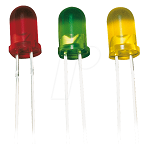
\includegraphics{fig/LEDperur}
  \caption{LEDS}
  \label{fig:LEDS}
\end{figure}

A LED (light-emitting diode) is used like a small light bulb, but is in fact a semiconductor, since it only lets current flow in one direction, from the anode to the cathode. It is used for many purposes in today's society, especially for lighting, regular light bulbs and Christmas lights, but also for back light in televisions. When working with Arduino you can make this small LED to light up constantly or to flash, depending on what purpose it serves. 

In this project the LED, well in fact there are three LED's (green, yellow and red), their purpose is to indicate whether the radar is on, off or loading, depending on the state of the push button. 

\subsection{RGB LED}

\begin{figure} [h!]
\centering
  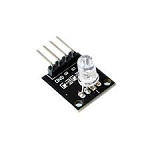
\includegraphics{fig/RGBLED}
  \caption{RGB LED}
  \label{fig:RGBLED}
\end{figure}

A RGB LED is much like a regular LED, but the main difference being that the RGB LED can change colour, meaning that it consists of three LED's with the standard colours red, green and blue. The brightness of each LED decides the colour of the LED, much like mixing paint, but using light instead of paint. 

The RGB LED used indicates at what distance the object detected by the Ultra Sonic is, so if the light of the RGB LED turns red the object is closer than 10 cm, if it turns green the object is between 10 cm to 100 cm and when it's blue the object is at a distance of a 100 cm or more.  

\subsection{Push button}

\begin{figure} [h!]
\centering
  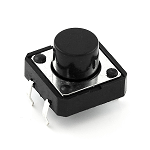
\includegraphics{fig/Pushbutton}
  \caption{Push button}
  \label{fig:Pushbutton}
\end{figure}

A push button reassembles a light switch in our home. When the button is not pressed it does not let any current through it, known as state HIGH in the programming. When the button gets pressed, it lets current flow through it, much like when a light switch is on, the state is known as LOW. 

The purpose of the button used is to turn the radar on and off, that means when the radar is off the red LED is lit and nothing moves. And when the button is pressed, the green LED is lit and the Radar is moving.

\subsection{LCD display}

\begin{figure} [h!]
\centering
  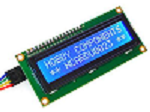
\includegraphics{fig/LCDdisplay}
  \caption{LCD Display}
  \label{fig:LCDdisplay}
\end{figure}  

The LCD display (liquid crystal display) is a very common thing, displays are used in everything from televisions to cell phones. The one for the Arduino is a very simple one, it doesn't come with colour, meaning the writing is white, and it is only capable of writing two lines, containing 16 signs in each line, it mostly resembles the old cell phones.   

Regarding the project, when the radar is turned off the display reads ``Radar project version $2.0$''. When turning the radar on the display clears and starts displaying the direction of the Servo Motor and Ultra Sonic. When the Ultra Sonic detects an object, the display shows at what distance the object is and at what angle from the radar. It also displays the temperature measured, by the temperature measurer, since the temperature has an effect on the speed of sound. 

\subsection{Temperature sensor}

\begin{figure} [h!]
\centering
  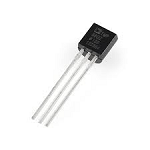
\includegraphics{fig/Temperaturesensor}
  \caption{Temperature sensor}
  \label{fig:temperaturesensor}
\end{figure} 

The temperature sensors job is to measure the temperature of the surroundings, since the speed of sound and temperature go hand in hand. 

\subsection{Servo motor}

\begin{figure} [h!]
\centering
  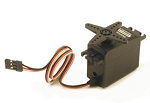
\includegraphics{fig/Servomotor}
  \caption{Servo motor}
  \label{fig:servo}
\end{figure} 

A servo motor is based on an Arduino library, which is included in the Arduino, the library is the used in the programming. On the hardware part, the servo motor has integrated gears and shaft, which allows it to be controlled precisely. The standard servo motor can be positioned at various angles between $0$ to $180$ degrees. 

The purpose of the Servo Motor is to turn the Ultrasonic sensor in an arc of $180$ degrees, from left to right and back. Its job is also to let the user and Arduino know at all times at what angle it's located. This information is used to tell at what angel an object is located. 


\subsection{Ultrasonic sensor}

\begin{figure} [h!]
\centering
  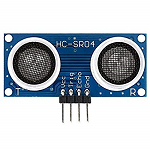
\includegraphics{fig/Ultrasonicsensor}
  \caption{Ultrasonic sensor}
  \label{fig:ultrasonic}
\end{figure}

The Ultrasonic sensor is based on sonar technology and can determine the distance of an object, with a range of $2 cm$ to $400 cm$. It doesn't get affected by sunlight and comes as a complete module, including the transmitter and receiver.  

In this case the ultrasonic sensor is placed on the moving servo motor, so it can detect objects in a 180-degree radius, thereby being able to see what is in front, it is the key component of the radar. By detecting an object and at what distance, it gives us an idea of where and how close in front of us an object is located.   

\subsection{Resistors}

\begin{figure} [h!]
\centering
  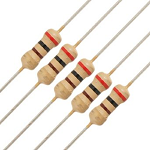
\includegraphics{fig/Resistor}
  \caption{Resistors}
  \label{fig:Resistors}
\end{figure}

The resistors help control the current flowing to different components, meaning the limit the amount of current flowing to the components. This becomes much needed when working with highly current sensitive components, like the LED's, which can only withstand $2 V$. However, it is also used in front of the push button to direct the current, to detect if the button is pressed down or not.

\section{Complete circuit}

\begin{figure} [h!]
\centering
  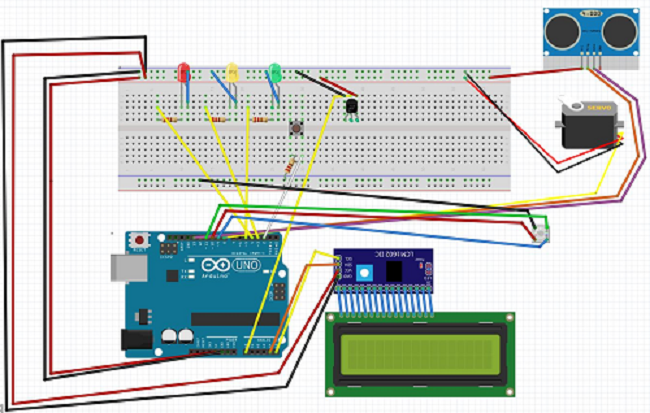
\includegraphics [width=\linewidth]{fig/Arduinoboard}
  \caption{Arduino drawing}
  \label{fig:Arduinoboard}
\end{figure}

On the picture it looks like everything is connected to each other and in a way it is, since the board itself is what brings everything together. But we can simplify it into this electrical drawing: 

\newpage

\begin{figure} [h!]
\centering
  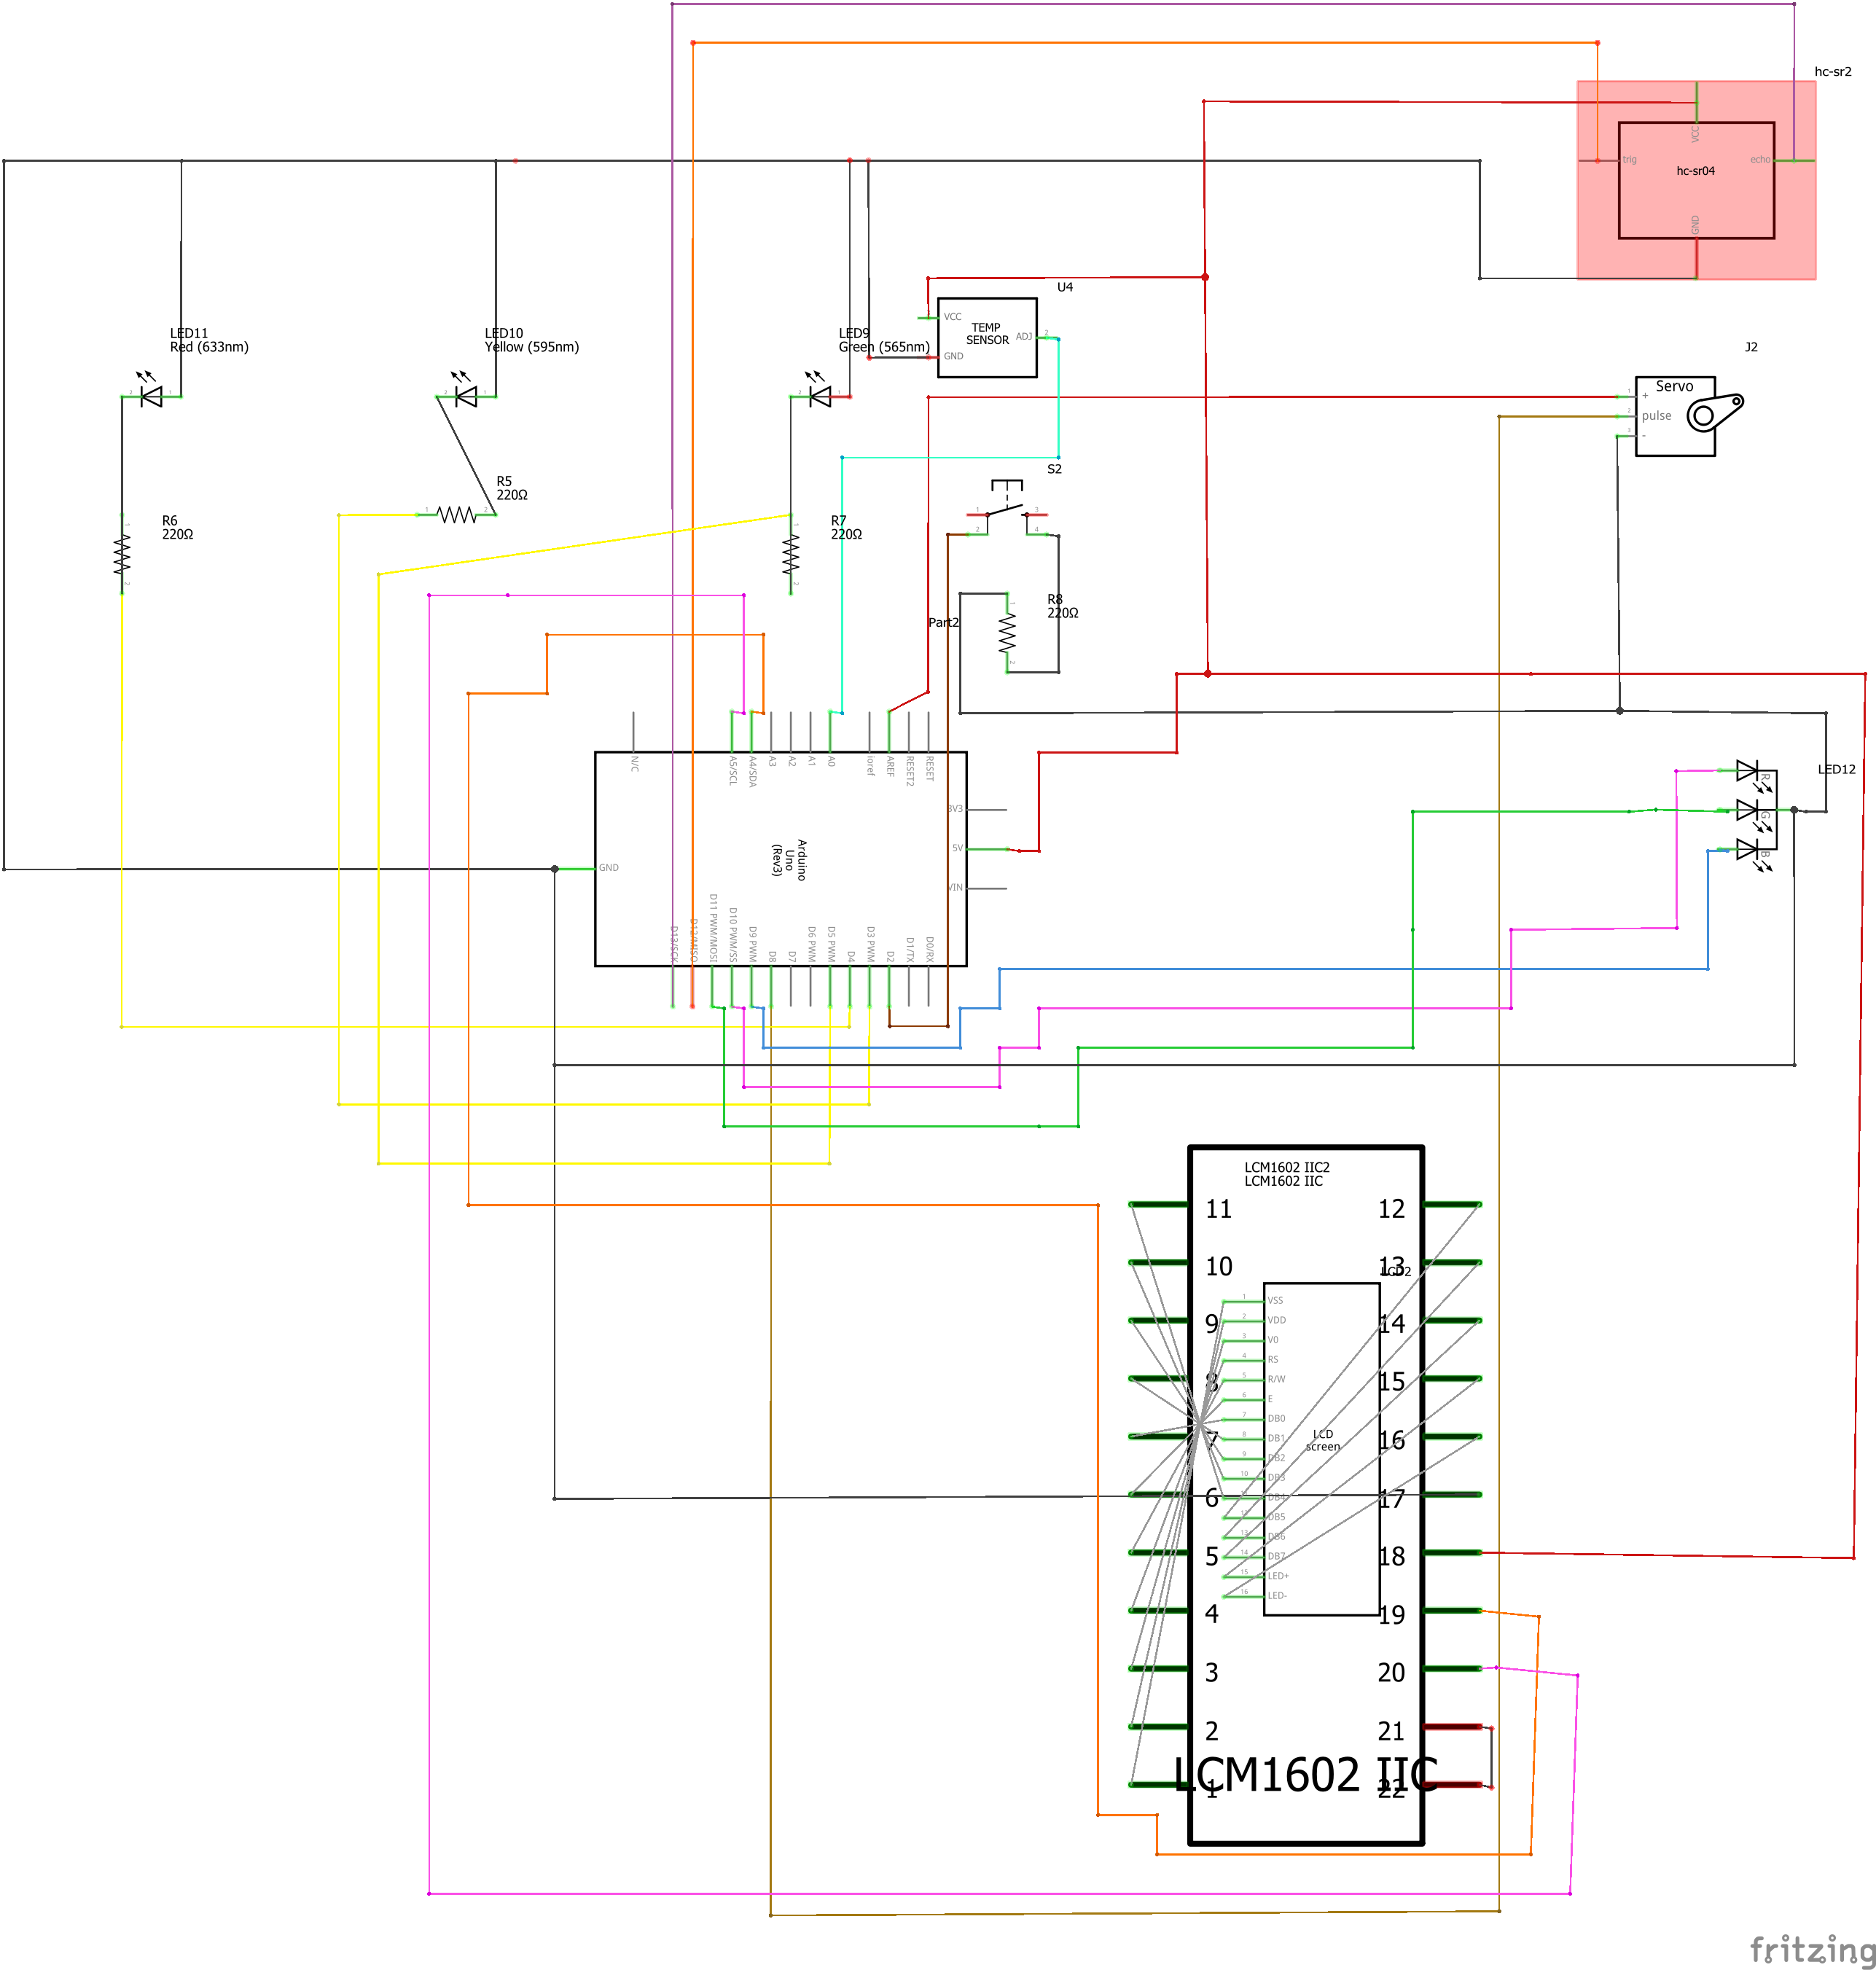
\includegraphics [width=\linewidth]{fig/Circuittekning}
  \caption{Circuit drawing}
  \label{fig:Circuitdrawing}
\end{figure}

As we can see the circuit board has been left out, and the individual components are all connected directly to the Arduino.  

OBS! The LCD display and the LCD controller are drawn as two components, but in this project they are one unit, so the non-important wires are grey, while the four wires connecting the LCD unit to the Arduino are the important ones. 
\chapter{How it's done}
Describing the process from start to finish, and the challenges we met along. 

The biggest challenge/uncertainty was to get the components in time. We had to order some components online, since the university did not have them in stock. We ordered the Ultra Sonic, LCD Display and RGB LED module form China. 

So while waiting for these components, we decided to attach and program the other components, which we already had. Like the three LED’s and belonging resistors, the servo motor and the button and to get them to function properly. 

So to start with, we got the LED lighting up with the press of the button and to stay on until the button was pressed again. Adding a second LED, so when the button was pressed on, the green LED ``lighted up'' and when the button was off, the red LED ``light'' up. This button function was then applied to every component throughout the project, more on this later. We then added the Servo motor and got it running smoothly. It was then added to the button function, turning on and off with the LED's. By now the components started arriving from Chine, starting out with the LCD display. Getting this to work properly was a small challenge, especially when rewriting itself, it showed to be challenging to get it to clear itself at the right time. Shortly after the RGB LED and the Ultra Sonic where attached, here the most challenging problem being the Ultra Sonic. The challenge was to get the programming in place for the Ultra Sonic, so that the Servo motor, which it is attached to, still was running smoothly. The Servo motor kept waiting for the Ultra Sonic, since the Ultra Sonic did not receive a signal back and therefore stalled the entire radar and made it not run fluidly.
\chapter{Code}

\section{Arduino Enviroment}

\subsection{Arduino Coding Environment}
To write code for Arduino devices, you need an IDE\footnote{Integrated development environment}. An IDE normally consists of a source code editor, build automation tools, and a debugger.  

The most popular IDE is Arduino IDE, which is very beginner friendly, but it has it's weaknesses when it comes to writing code, for instance the lacking of $intelliSense$\footnote{IntelliSense is a code-completion aid that includes a number of features: List Members, Parameter Info, Quick Info, and Complete Word.}. This is not an issue when making a small project, like making a LED blink. But when it comes to bigger projects, which have many components and 3rd party libraries, coding becomes very hard without intelliSense. Another disadvantage with Arduino IDE, is when working with many files. The more files the project has the more complicated it becomes to locate them, since it is all set up like a large document instead of small subsections. A small example of this \ref{fig:example}

\newpage

\begin{figure}[!h]
    \centering
    \subfloat[Arduino IDE]{{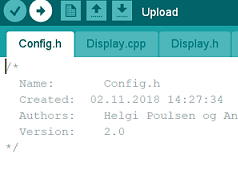
\includegraphics[width=5cm]{fig/arduinofiles} }}%
    \qquad
    \subfloat[Visual Studio 2017]{{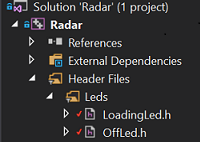
\includegraphics[width=5cm]{fig/vsfiles} }}%
    \caption{Difference in file structure}%
    \label{fig:example}%
\end{figure} 
 

For these reasons and others, Visual Studio was used to create this project.

\subsection{Arduino code}
The Arduino language is merely a set of $C/C++$ functions that can be called from your code. All standard $C$ and $C++$ constructs supported by $avr-g++$ should work in Arduino.\footnote{\url{https://www.arduino.cc/en/Main/FAQ}}

Arduino uses sketches. A sketch is the name that Arduino uses for a program. It's the unit of code that is uploaded to and run on an Arduino board.

Every project must have one main sketch file, which must be an $.INO$ file. This is the file containing the $setup()$ and $loop()$ functions. The $setup()$ runs only once, when the Arduino is powered up. After $setup()$, the $loop()$ function runs  over and over. This means that when $\}$ is reached, it starts from the top again.

$.CPP$ and $.H$ files can also be used and is recommended, since it gives you more control and overview.

\newpage

\section{Libraries}
Libraries are files written in C or C++, which provide your sketches with extra functionality. More information about them can be found at \url{https://www.arduino.cc/en/Main/Libraries}, where even a template is provided so that the user can write his own library.

In this project we used a few libraries:
\begin{multicols}{2}
\begin{itemize}
	\item Servo \textit{Servo}
	\item LiquidCrystal\_I2C \textit{Display}
	\item NewPing \textit{Ultrasonic}	
	\item Wire \textit{Display}	
\end{itemize}
\end{multicols}

\section{Radar.ino}
This is the main file in the project. Here we have included all the header files and created objects that are needed, like the $servo$ and $lcd$ objects that come from the $servo$ and $LiquidCrystal\_I2C$ libraries.

\subsection{void setup()}
\lstinputlisting[language=c++,firstline=33, lastline=51]{Backmatter/Code/Radar.ino}

\subsubsection{Serial.begin(9600)}
Sets the data rate in $bits per second (baud)$ for serial data transmission. For communicating with the computer. The rate set is $9600$.
\subsubsection{Serial.println()}
The serial.println() functions are used for printing the data to the serial port. In this case it is used to get the data into a $Excel$ spreadsheet via a software called $PLX-DAQ$\footnote{PLX-DAQ is a Parallax microcontroller data acquisition add-on tool for Microsoft Excel} for the tests to measure the accuracy of the ultrasonic sensor. More information about $PLX-DAQ$ can be found on \href{https://www.parallax.com/downloads/plx-daq}{PLX-DAQ}  

\subsubsection{Servo}
We initialize the servo here by attaching it to a pin and setting it to position $0$.

\subsubsection{load.blink()}
This is just making the yellow led blink fast multiple times. This just gives the user the sensation that everything is starting up.

\subsubsection{lcd}
here we initialize the lcd display and turn it on. 
$display.intro(lcd)$ is the function that shows the intro screen.

\subsection{void loop()} \label{voidloop}
\lstinputlisting[language=c++,firstline=53, lastline=57]{Backmatter/Code/Radar.ino}

Here is where the magic happens. In our $loop()$, we only have one function, that controls everything.

$run(servo, lcd)$ takes two arguments, the servo object and the lcd object. 

\section{Classes}
We have created a class for each component(sensor,motor,led), since the main purpose of C++ programming is to add object orientation to the C programming language. This gives us much more flexibility with the project and makes it much easier to expand. Each class is also in its own header file. Our classes are:
\begin{itemize}
  \item UltraSonicClass
  \item TemperatureClass
  \item ServoMotorClass
  \item SerialPrintClass
  \item PowerOnOffClass
  \item DisplayClass
  \item LedClass
  \begin{itemize}
     \item LoadingLedClass
     \item OnLedClass
     \item OffLedClass
   \end{itemize}
  \item RGBLedClass
\end{itemize}

We use hierarchical inheritance for the led classes. We wanted to add a factory method design pattern\footnote{\url{https://www.tutorialspoint.com/design_pattern/factory_pattern.htm}} to the led classes, but we encountered some strange object problems.  

\section{Config.h}
The config header file contains the constants for the digital and analog pins. Here we use namespace\footnote{A namespace is a declarative region that provides a scope to the identifiers (names of the types, function, variables etc.) inside it.}

\section{Functions}
This project contains lots of classes and functions. Here we will take a closer look at some of the more complicated and important ones.

\subsection{void run(Servo s, LiquidCrystal\_I2C lcd)\ref{appendix:PowerOnOff}}
As mentioned in \ref{voidloop}, this is the main function. 

$void run(Servo s, LiquidCrystal\_I2C lcd)$ is the button. If turned on, turn the servo, measure  temperature, measure distance and so on. If off, stop everything, turn the the red led on and display the into on the display.

Since the code is heavily commented, to make it as easy to understand as possible, the need to explain each line is not necessary. 

To get the button to work as intended was more complicated that it seemed. 
\newpage

The basic principle of it\ref{fig:btnDiagram}:
\begin{figure}
  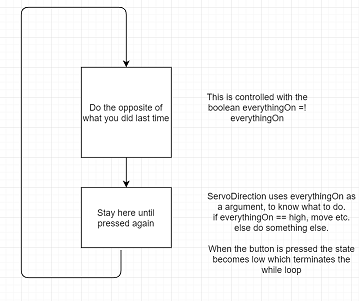
\includegraphics[width=\linewidth]{fig/buttonDiagram}
  \caption{Button diagram}
  \label{fig:btnDiagram}
\end{figure}

\subsection{void servoDirection(Servo s, int state, LiquidCrystal\_I2C lcd)\ref{appendix:PowerOnOff}}
In $void servoDirection(Servo s, int state, LiquidCrystal\_I2C lcd)$.
we check if the state is $HIGH$, then for every 10 counter degrees, we set the temperature and speed of sound. We do this since the temperature module is not stable enough. Then we set the distance in $centimeters$ and then showing the distance with the rgb module and print the important information on the display.

We use a $if$ statement with the argument $up$, that is a boolean, to decide which way the servo goes. If up is true then go from $min$ to $max$, else go from $max$ to $min$. 

The $counter$ is the servo position. So when $counter$ reaches $max$, we set up $= false$.

the string $leftRight$ and integer $test$ are only used for $serialPrint$\ref{appendix:SerialPrint}.

$sm.rotate$\ref{appendix:ServoMotor} is the function that rotates the servo. It takes $servo$ and $counter$ as arguments.

\subsection{void setSpeedOfSound(int temperature)\ref{appendix:UltraSonic}}
To set the speed of sound with temperature, we need to use the speed of sound formula:
\begin{equation}
c = 331.3 \times \sqrt{\frac{\vartheta + 273.15}{273.15}} = 331.3 \times \sqrt{1 + \frac{\vartheta}{273.15}}
\end{equation}
A simplified formula can be used for $\ang{+35} C to \ang{-35} C$

Speed of sound in air in m/s:
\begin{equation}
c=331.3 + 0.6 \times \vartheta
\end{equation}
To make our calculations light weight as possible, we used the the simplified formula.

\subsection{void setDistance(float speedOfSound)\ref{appendix:UltraSonic}}
We found a very good library, $NewPing$, that can measure the distance for the ultrasonic sensor. We decided not to use it since it doesn't take speed of sound as argument and found it better for the project to write the code ourselves. 

We show how to use it in the inline comments if the reader wants to use it instead of our code.

First we set the trigger pin to $LOW$ and make a $4$ microseconds delay to ensure a clean $HIGH$ pulse, then the sensor is triggered by a $HIGH$ pulse of $10$ microseconds.

$duration$ is the time in microseconds from the sending of the ping to the reception of its echo off of an object.

Then we convert the time into $cm$ 
\begin{equation}
distance = \frac{duration \times \frac{speedOfSound}{1000}}{2} 
\end{equation}

\subsection{void setTemperature()\ref{appendix:Temperature}}
To turn the 10-bit analog reading into a temperature:

Formula that converts the number $0/1023$ from Analog ADC input into $0-5000mV(=5V)$:

First we read the analog pin, then:
\begin{equation}
voltage = reading \times 5.0
\end{equation}
then:
\begin{equation}
voltage = \frac{voltage}{1024}
\end{equation}

Convert to Celsius:
\begin{equation}
temperatureCelsius = (voltage - 0.5) \times 100
\end{equation}



\chapter{Ultrasonic test results}

\section{Range test (No motion)} 

\begin{figure} [h!]
  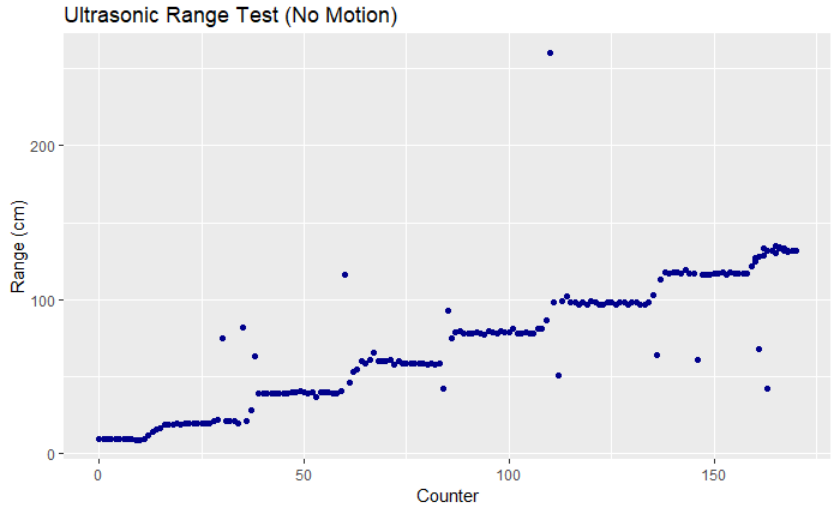
\includegraphics[width=\linewidth]{fig/test1}
  \caption{Ultrasonic range test (no motion)}
  \label{fig:test1}
\end{figure}

We did a ultrasonic range test where we placed a object in front of the ultrasonic sensor and moved it back \ref{fig:test1}. The test result shows that we got some outliers, but overall the ultrasonic sensor was fairly accurate.

\newpage

\section{Ultrasonic range test (motion)} 

\begin{figure} [h!]
  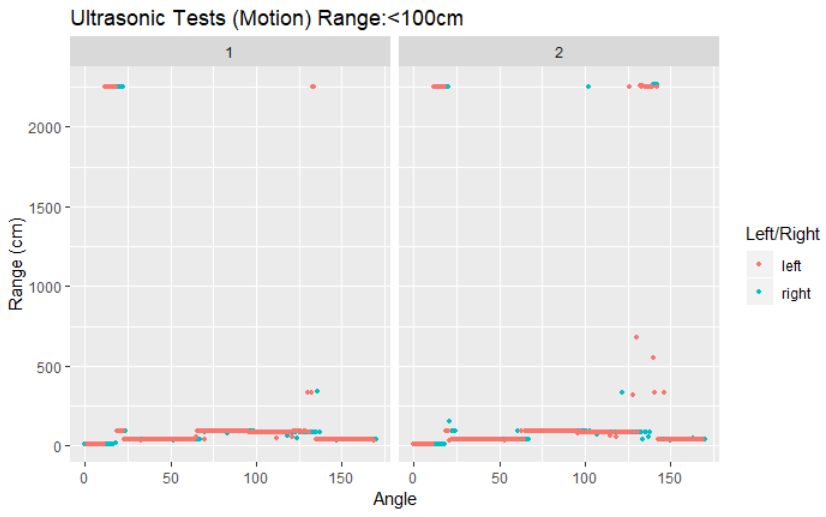
\includegraphics[width=\linewidth]{fig/test2}
  \caption{Ultrasonic range test (motion)}
  \label{fig:test2}
\end{figure}

This test shows how accurate the sensor is when moving from $0$ to $170$ (right) then $170$ to $0$ (left) two times, $Test 1$ and $Test 2$. As seen on \ref{fig:test2}.

The test\ref{fig:test2} should show us again that the sensor is accurate enough for us to work with, even though we got some strange outliers, like in $Test 2$ between Angle $130$ and $150$. The outliers that are $2500 cm$ is when the sensor didn't hit an object. 

\newpage

\section{Ultrasonic range test (motion) Range:<100 cm} 

\begin{figure} [h!]
  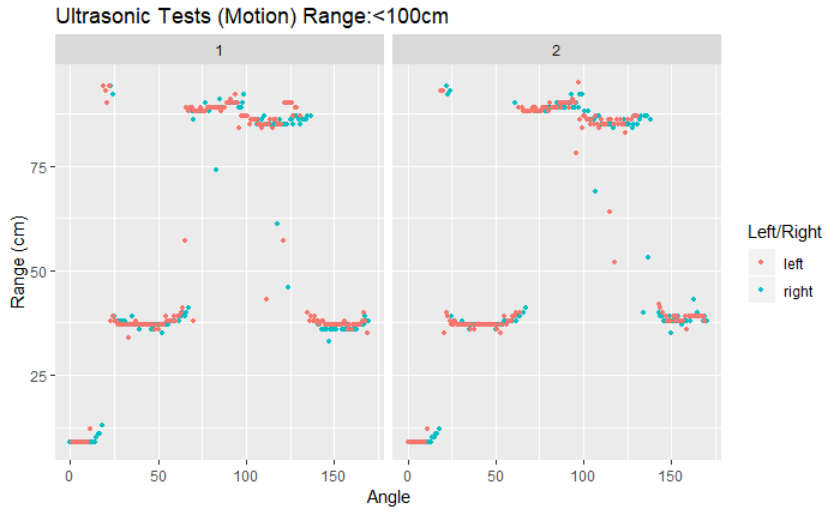
\includegraphics[width=\linewidth]{fig/test3}
  \caption{Ultrasonic range test (motion) Range:<100 cm}
  \label{fig:test3}
\end{figure}

In \ref{fig:test3} we only show everything that is below $100 cm$. This is to show a better image of the results.

\newpage

\section{Ultrasonic range tests separated (motion) Range:<100 cm} 

\begin{figure}[!h]
    \centering
    \subfloat[Test 1]{{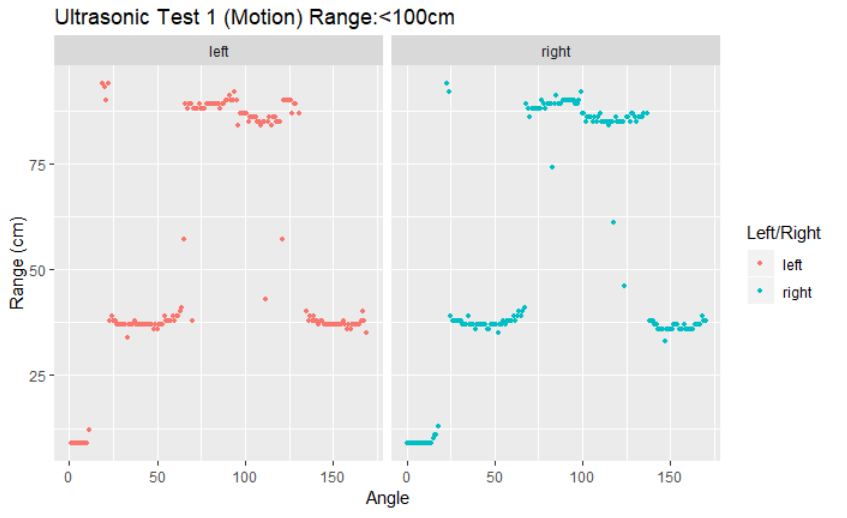
\includegraphics[width=5cm]{fig/test4} }}%
    \qquad
    \subfloat[Test 2]{{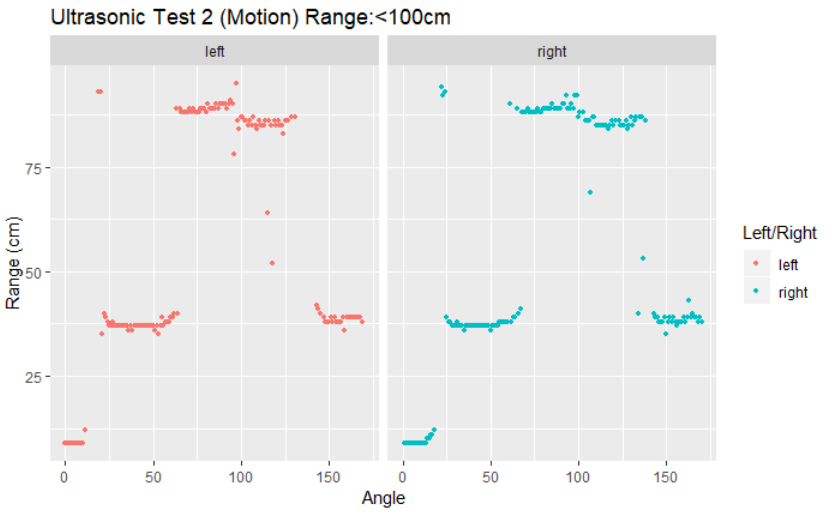
\includegraphics[width=5cm]{fig/test5} }}%
    \caption{Ultrasonic range tests separated (motion) Range:<100 cm}%
    \label{fig:test45}%
\end{figure} 

Here everything is separated. If the ultrasonic sensor was $100\%$ accurate, all the four images should look the same. As we can see to look quite similar, at least similar enough for us to be happy with the test results. 

We can also point out that a reason for the test results not looking exactly the same where the temperature readings. Sometimes we also got strange temperature readings and since we took a reading every $10$ degree, this could have a small effect on the results.

\chapter{The results}
The complete radar is now serving its goal, but the one thing not working perfectly is the Ultrasonic sensor. There seems to be some kind of error in the code, so when the receiver doesn't receive an echo, the radar glitches for an instant, before continuing on its arc. We discovered that if we used the pre-set library, the glitch did not appear, but that library didn't take in account the temperature. Therefore, we decided to continue with our own code, instead of trying to change the library, also time was becoming an issue.  

The test we made proved to be satisfying, even though there were some slight errors because of the fluctuations of the temperature sensor, these can be seen on the graphs shown earlier. Since the main principle of the radar is working and it's accuracy is precise enough for this project, the radar is found satisfying. 

If we were going to continue working on the radar project, of course fixing the glitch would be our first priority, but adding an OLED display would be very beneficial. Sine the OLED display can give the user a graphical view of the measurements, meaning it looks more like the output you get from an actual radar. Also, it would be highly beneficial to design a surface or box, so that such things as wires, breadboard and Arduino Uno aren't exposed, hence it would look more like a small gadget that you could buy at a local store. It could potentially be a small toy for children, from the age of 10 or so. 
\chapter{Conclusion}
Looking back on the project we have been through a learning curve, a learning curve involving Arduino software and hardware, especially getting hardware and software working together has been a steep learning curve, since it has proven to be hard to get all the components working together and as intended, since the coding didn't always seem logical. 

The majority of the hardware components are fairly simple, but when looking at the LCD display and the Ultrasonic sensor proved to be a challenge to understand their nature. Regarding the coding the challenge again showed itself regarding the same components as with the hardware, but here especially the programming of the push button proved to be a challenge, since it isn't logical or in other words it isn't a switch, but we want it to work as one. 

The radar itself is now up and running, it doesn’t work perfectly as a modern radar, since it’s a school project and with the time given there is no chance to get it to the standards of a modern radar. But as a school project it is satisfying, and we are able to show the principle of a radar and we have gotten some insight in how Arduino can be used in the modern society

\begin{appendices}

\appendix
\chapter{Plots for tests}
\lstinputlisting[language=R]{Backmatter/TestResults/TestResults.rmd}

\newpage


\chapter{Code}
\section{Radar.ino}
\lstinputlisting[language=c++]{Backmatter/Code/Radar.ino}

\newpage

\section{PowerOnOff}
\label{appendix:PowerOnOff}
\lstinputlisting[language=C++]{Backmatter/Code/PowerOnOff.h}
\lstinputlisting[language=C++]{Backmatter/Code/PowerOnOff.cpp}

\newpage

\section{ServoMotor}
\label{appendix:ServoMotor}
\lstinputlisting[language=C++]{Backmatter/Code/ServoMotor.h}
\lstinputlisting[language=C++]{Backmatter/Code/ServoMotor.cpp}

\newpage

\section{UltraSonic}
\label{appendix:UltraSonic}
\lstinputlisting[language=C++]{Backmatter/Code/UltraSonic.h}
\newpage
\lstinputlisting[language=C++]{Backmatter/Code/UltraSonic.cpp}

\newpage

\section{Temperature}
\label{appendix:Temperature}
\lstinputlisting[language=C++]{Backmatter/Code/Temperature.h}
\newpage
\lstinputlisting[language=C++]{Backmatter/Code/Temperature.cpp}

\newpage

\section{Display}
\label{appendix:Display}
\lstinputlisting[language=C++]{Backmatter/Code/Display.h}
\newpage
\lstinputlisting[language=C++]{Backmatter/Code/Display.cpp}

\newpage

\section{RGBLed}
\label{appendix:RGBLed}
\lstinputlisting[language=C++]{Backmatter/Code/RGBLed.h}
\newpage
\lstinputlisting[language=C++]{Backmatter/Code/RGBLed.cpp}

\newpage

\section{Leds}
\label{appendix:Leds}
\lstinputlisting[language=C++]{Backmatter/Code/Led.h}
\lstinputlisting[language=C++]{Backmatter/Code/Led.cpp}
\newpage
\lstinputlisting[language=C++]{Backmatter/Code/OnLed.h}
\lstinputlisting[language=C++]{Backmatter/Code/OnLed.cpp}

\lstinputlisting[language=C++]{Backmatter/Code/OffLed.h}
\newpage
\lstinputlisting[language=C++]{Backmatter/Code/OffLed.cpp}

\lstinputlisting[language=C++]{Backmatter/Code/LoadingLed.h}
\lstinputlisting[language=C++]{Backmatter/Code/LoadingLed.cpp}

\newpage

\section{SerialPrint}
\label{appendix:SerialPrint}
\lstinputlisting[language=C++]{Backmatter/Code/SerialPrint.h}
\newpage
\lstinputlisting[language=C++]{Backmatter/Code/SerialPrint.cpp}

\newpage

\section{Config}
\label{appendix:Config}
\lstinputlisting[language=C++]{Backmatter/Code/Config.h}
\end{appendices}



\end{document}